\documentclass[journal,12pt,twocolumn]{IEEEtran}
\usepackage{setspace}
\usepackage{gensymb}
\singlespacing
\usepackage[cmex10]{amsmath}
\usepackage{amsthm}
\usepackage{mathrsfs}
\usepackage{txfonts}
\usepackage{stfloats}
\usepackage{bm}
\usepackage{cite}
\usepackage{cases}
\usepackage{subfig}
\usepackage{longtable}
\usepackage{multirow}
\usepackage{enumitem}
\usepackage{mathtools}
\usepackage{steinmetz}
\usepackage{tikz}
\usepackage{circuitikz}
\usepackage{verbatim}
\usepackage{tfrupee}
\usepackage[breaklinks=true]{hyperref}
\usepackage{graphicx}
\usepackage{tkz-euclide}
\usetikzlibrary{calc,math}
\usepackage{listings}
\usepackage{color}                                            %%
\usepackage{array}                                            %%
\usepackage{longtable}                                        %%
\usepackage{calc}                                             %%
\usepackage{multirow}                                         %%
\usepackage{hhline}                                           %%
\usepackage{ifthen}                                           %%
\usepackage{lscape}     
\usepackage{multicol}
\usepackage{chngcntr}
\DeclareMathOperator*{\Res}{Res}
\renewcommand\thesection{\arabic{section}}
\renewcommand\thesubsection{\thesection.\arabic{subsection}}
\renewcommand\thesubsubsection{\thesubsection.\arabic{subsubsection}}
\renewcommand\thesectiondis{\arabic{section}}
\renewcommand\thesubsectiondis{\thesectiondis.\arabic{subsection}}
\renewcommand\thesubsubsectiondis{\thesubsectiondis.\arabic{subsubsection}}
\hyphenation{op-tical net-works semi-conduc-tor}
\def\inputGnumericTable{}                                 %%
\lstset
{
%language=C,
frame=single, 
breaklines=true,
columns=fullflexible
}
\begin{document}
\newtheorem{theorem}{Theorem}[section]
\newtheorem{problem}{Problem}
\newtheorem{proposition}{Proposition}[section]
\newtheorem{lemma}{Lemma}[section]
\newtheorem{corollary}[theorem]{Corollary}
\newtheorem{example}{Example}[section]
\newtheorem{definition}[problem]{Definition}
\newcommand{\comb}[2]{{}^{#1}\mathrm{C}_{#2}}
\newcommand{\BEQA}{\begin{eqnarray}}
\newcommand{\EEQA}{\end{eqnarray}}
\newcommand{\define}{\stackrel{\triangle}{=}}
\bibliographystyle{IEEEtran}
\raggedbottom
\setlength{\parindent}{0pt}
\providecommand{\mbf}{\mathbf}
\providecommand{\pr}[1]{\ensuremath{\Pr\left(#1\right)}}
\providecommand{\qfunc}[1]{\ensuremath{Q\left(#1\right)}}
\providecommand{\sbrak}[1]{\ensuremath{{}\left[#1\right]}}
\providecommand{\lsbrak}[1]{\ensuremath{{}\left[#1\right.}}
\providecommand{\rsbrak}[1]{\ensuremath{{}\left.#1\right]}}
\providecommand{\brak}[1]{\ensuremath{\left(#1\right)}}
\providecommand{\lbrak}[1]{\ensuremath{\left(#1\right.}}
\providecommand{\rbrak}[1]{\ensuremath{\left.#1\right)}}
\providecommand{\cbrak}[1]{\ensuremath{\left\{#1\right\}}}
\providecommand{\lcbrak}[1]{\ensuremath{\left\{#1\right.}}
\providecommand{\rcbrak}[1]{\ensuremath{\left.#1\right\}}}
\theoremstyle{remark}
\newtheorem{rem}{Remark}
\newcommand{\sgn}{\mathop{\mathrm{sgn}}}
\providecommand{\abs}[1]{\vert#1\vert}
\providecommand{\res}[1]{\Res\displaylimits_{#1}} 
\providecommand{\norm}[1]{\lVert#1\rVert}
%\providecommand{\norm}[1]{\lVert#1\rVert}
\providecommand{\mtx}[1]{\mathbf{#1}}
\providecommand{\mean}[1]{E[#1]}
\providecommand{\fourier}{\overset{\mathcal{F}}{ \rightleftharpoons}}
\providecommand{\ztransform}{\overset{\mathcal{Z}}{ \rightleftharpoons}}
%\providecommand{\hilbert}{\overset{\mathcal{H}}{ \rightleftharpoons}}
\providecommand{\system}{\overset{\mathcal{H}}{ \longleftrightarrow}}
%\newcommand{\solution}[2]{\textbf{Solution:}{#1}}
\newcommand{\solution}{\noindent \textbf{Solution: }}
\newcommand{\cosec}{\,\text{cosec}\,}
\providecommand{\dec}[2]{\ensuremath{\overset{#1}{\underset{#2}{\gtrless}}}}
\newcommand{\myvec}[1]{\ensuremath{\begin{pmatrix}#1\end{pmatrix}}}
\newcommand{\mydet}[1]{\ensuremath{\begin{vmatrix}#1\end{vmatrix}}}
\numberwithin{equation}{subsection}
\makeatletter
\@addtoreset{figure}{problem}
\makeatother
\let\StandardTheFigure\thefigure
\let\vec\mathbf
\renewcommand{\thefigure}{\theproblem}
\def\putbox#1#2#3{\makebox[0in][l]{\makebox[#1][l]{}\raisebox{\baselineskip}[0in][0in]{\raisebox{#2}[0in][0in]{#3}}}}
\def\rightbox#1{\makebox[0in][r]{#1}}
\def\centbox#1{\makebox[0in]{#1}}
\def\topbox#1{\raisebox{-\baselineskip}[0in][0in]{#1}}
\def\midbox#1{\raisebox{-0.5\baselineskip}[0in][0in]{#1}}
\vspace{3cm}


\title{EE3900 Gate Assignment-2}
\author{V Rahul - AI20BTECH11030}
\maketitle
\newpage
\bigskip
\renewcommand{\thefigure}{\theenumi}
\renewcommand{\thetable}{\theenumi}
Download all python codes from 
\begin{lstlisting}
    https://github.com/vrahul02/EE3900/tree/main/Gate-Assignment-2/Codes
\end{lstlisting}
%
and latex-tikz codes from 
%
\begin{lstlisting}
    https://github.com/vrahul02/EE3900/tree/main/Gate-Assignment-2/Gate-Assignment-2.tex
\end{lstlisting}
\section*{Problem Gate EC-2006 Q.53}
A system with input $x[n]$ and output $y[n]$ is given as $y[n]=\left(\sin{\frac{5}{6}\pi n}\right) x(n)$. The system is:\\
\begin{enumerate}
    \item linear, stable and invertible
    \item non-linear, stable and non-invertible
    \item linear, stable and non-invertible
    \item linear, unstable and invertible
\end{enumerate}
\section*{Solution}
For linearity,\\
\begin{align}
    x(n)&=x_1(n)\\
    \implies y_1(n)&=\left(\sin{\frac{5}{6}\pi n}\right)  x_1(n)\\
    x(n)&=x_2(n)\\
    \implies y_1(n)&=\left(\sin{\frac{5}{6}\pi n}\right) x_1(n)
\end{align}
If
\begin{align}
    x(n)&=x_1(n)+x_2(n)\\
    \implies y(n)&=\left(\sin{\frac{5}{6}\pi n}\right) x_1(n)+\left(\sin{\frac{5}{6}\pi n}\right) x_1(n)\\
    y(n)&=\left(\sin{\frac{5}{6}\pi n}\right)  \left(x_1(n)+x_2(n)\right)\\
    \therefore y(n)&=y_1(n)+y_2(n)
\end{align}
Thus, it is a linear system\\
Also for a bounded input we get bounded output. Thus it is a stable system.\\
Now if
\begin{align}
    n&=0\\
    y(n)&=0
\end{align}
And
\begin{align}
    n&=2\\
    y(n)&=0
\end{align}
For different values of input, output is same. Thus the system is non-invertible\\
\begin{table}[!ht]
\begin{tabular}{|l|l|}
\hline
Linearity     & Linear         \\ \hline
Stability     & Stable         \\ \hline
Invertibility & Non-Invertible \\ \hline
\end{tabular}
\end{table}\\
Thus option 3) is correct\\
Numerical examples:\\
\begin{enumerate}[label= (\alph*)]
    \item $x(n)=1$
    \begin{align}
        y(n)=\sin{\frac{5}{6}\pi n}
    \end{align}
    \begin{figure}[!ht]
    \centering
    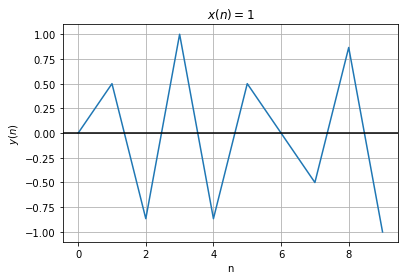
\includegraphics[width=\columnwidth]{Gate Assignment-2(1).png}
    \caption{Plot of output vs n when $x(n)=1$}
    \label{a}
    \end{figure}
    \item $x(n)=n$
    \begin{align}
        y(n)=\left(\sin{\frac{5}{6}\pi n}\right)n
    \end{align}
    \begin{figure}[!ht]
    \centering
    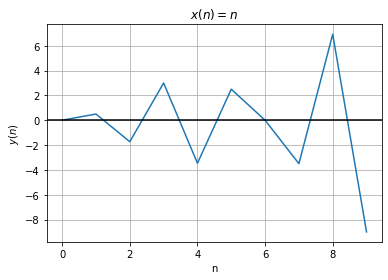
\includegraphics[width=\columnwidth]{Gate Assignment-2(2).png}
    \caption{Plot of output vs n when $x(n)=n$}
    \label{a}
    \end{figure}
\end{enumerate}
\end{document}